\documentclass[12pt,a4paper]{article}
\usepackage[utf8]{inputenc}
\usepackage[italian]{babel}
\usepackage{geometry}
\usepackage{graphicx}
\usepackage{listings}
\usepackage{xcolor}
\usepackage{hyperref}
\usepackage{booktabs}
\usepackage{tabularx}
\usepackage{fancyhdr}
\usepackage{float}

\geometry{margin=2.5cm}

\hypersetup{
    colorlinks=true,
    linkcolor=blue!60!black,
    urlcolor=blue!60!black,
    citecolor=blue!60!black
}

\lstset{
    basicstyle=\ttfamily\small,
    breaklines=true,
    frame=single,
    backgroundcolor=\color{gray!5},
    keywordstyle=\color{blue!70!black},
    commentstyle=\color{green!50!black},
    stringstyle=\color{red!60!black},
    showstringspaces=false,
    tabsize=2
}

\pagestyle{fancy}
\fancyhf{}
\fancyhead[L]{\small Shipping on the Air}
\fancyhead[R]{\small SAP - Assignment 1}
\fancyfoot[C]{\thepage}

\title{
    \textbf{Shipping on the Air} \\[0.5em]
    \large Assignment \#01 - Software Architecture and Platforms \\[0.3em]
    \normalsize A.Y. 2025/2026
}
\author{Fabio Vincenzi}
\date{\today}

\begin{document}

\maketitle
\tableofcontents
\newpage

% ============================================================
\section{Introduzione}
% ============================================================

Il progetto \textit{Shipping on the Air} realizza un sistema online per la consegna di pacchi tramite droni.
L'utente pu\`o richiedere la spedizione di un pacco specificando luogo di ritiro, luogo di consegna, peso e tempistica (immediata o programmata), e monitorare in tempo reale lo stato della consegna.

Il processo di sviluppo segue i seguenti principi:
\begin{itemize}
    \item \textbf{Domain-Driven Design} come approccio metodologico dall'analisi allo sviluppo;
    \item \textbf{Microservices} come stile architetturale;
    \item \textbf{Clean/Hexagonal Architecture} come struttura interna di ogni servizio.
\end{itemize}

% ============================================================
\section{Analisi}
% ============================================================

La Figura~\ref{fig:use-cases} mostra il diagramma dei casi d'uso del sistema.

\begin{figure}[H]
\centering
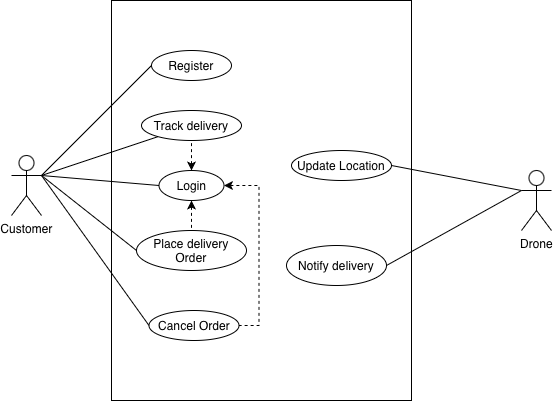
\includegraphics[width=0.65\textwidth]{../doc/analysis/use-cases.png}
\caption{Diagramma dei casi d'uso}
\label{fig:use-cases}
\end{figure}

\subsection{User Stories}

Le user stories catturano i requisiti funzionali dal punto di vista degli attori del sistema.

\begin{table}[H]
\centering
\small
\begin{tabularx}{\textwidth}{lX}
\toprule
\textbf{ID} & \textbf{User Story} \\
\midrule
US-1 & As a visitor, I want to register an account, so that I can use the delivery service. \\
US-2 & As a customer, I want to log in, so that I can place and manage orders. \\
US-3 & As a customer, I want to place a delivery order specifying pickup, delivery location and package weight, so that my package is delivered by drone. \\
US-4 & As a customer, I want to choose immediate or scheduled delivery, so that it fits my needs. \\
US-5 & As a customer, I want to see ETA before confirming, so that I can decide whether to proceed. \\
US-6 & As a customer, I want to cancel a pending order, so that I can change my mind before dispatch. \\
US-7 & As a customer, I want to track my delivery in real time, so that I know where my package is. \\
US-8 & As a customer, I want to see the ETA, so that I know when to expect my package. \\
US-9 & As a customer, I want to be notified when delivery is completed. \\
US-10 & As the system, I want to automatically assign the nearest available drone to a confirmed order. \\
US-11 & As the system, I want to receive real-time location updates from drones. \\
US-12 & As the system, I want to release a drone after delivery completion. \\
\bottomrule
\end{tabularx}
\caption{User Stories}
\end{table}

\subsection{Ubiquitous Language}

L'\textit{Ubiquitous Language} \`e il vocabolario condiviso tra esperti di dominio e sviluppatori, coerente all'interno di ogni Bounded Context.

\begin{table}[H]
\centering
\small
\begin{tabularx}{\textwidth}{lX}
\toprule
\textbf{Termine} & \textbf{Significato} \\
\midrule
Customer & Utente che richiede consegne tramite drone \\
Delivery Order & Richiesta di consegna: pacco, luoghi, tempistica, stato \\
Package & Oggetto da consegnare, caratterizzato da peso (kg) \\
Pickup Location & Luogo di ritiro (indirizzo + coordinate GPS) \\
Delivery Location & Luogo di consegna (indirizzo + coordinate GPS) \\
Drone & Veicolo aereo autonomo con capacit\`a di carico e autonomia limitata \\
Delivery & Trasporto di un pacco dal pickup al delivery location tramite drone \\
Route & Percorso calcolato dal pickup al delivery location \\
ETA & Tempo stimato di arrivo \\
Tracking & Monitoraggio real-time di posizione drone e stato consegna \\
\bottomrule
\end{tabularx}
\caption{Ubiquitous Language (estratto)}
\end{table}

\subsection{Quality Attribute Scenarios}

I Quality Attribute Scenarios (QAS) descrivono i requisiti non-funzionali in modo misurabile, secondo il formato a 6 parti.

\begin{table}[H]
\centering
\small
\begin{tabularx}{\textwidth}{llX}
\toprule
\textbf{QAS} & \textbf{Attributo} & \textbf{Scenario} \\
\midrule
QAS-1 & Performance & Il tracking restituisce la posizione GPS e ETA in meno di 1s, con aggiornamenti ogni 5s, sotto carico di 50 consegne attive. \\
QAS-2 & Availability & Il servizio ordini accetta e conferma ordini con disponibilit\`a del 99.9\%. \\
QAS-3 & Modifiability & L'integrazione di un nuovo modello di drone richiede modifiche in un solo servizio. \\
QAS-4 & Scalability & Il raddoppio degli ordini giornalieri non causa degrado di performance grazie allo scaling orizzontale indipendente per servizio. \\
\bottomrule
\end{tabularx}
\caption{Quality Attribute Scenarios}
\end{table}

\subsection{Acceptance Tests (BDD)}

Gli acceptance test sono scritti in formato Gherkin e implementati con \textbf{Cucumber}. Ogni scenario \`e collegato a step definitions Java che testano direttamente il layer application, senza necessit\`a di avviare i servizi HTTP.

\begin{lstlisting}[language={}]
Feature: Place delivery order

  Scenario: Successful immediate order
    Given I am a logged-in customer
    And at least one drone is available near the pickup area
    When I place a delivery order with:
      | pickup   | Via Roma 1, Cesena     |
      | delivery | Via Garibaldi 5, Forli |
      | weight   | 2.5 kg                 |
      | when     | immediate              |
    Then a delivery order is created in CONFIRMED status
    And I receive a confirmation with estimated delivery time

  Scenario: Weight exceeds limit
    Given I am a logged-in customer
    When I place an order with a package weighing 50 kg
    Then the order is rejected
\end{lstlisting}

% ============================================================
\section{Design Strategico (DDD)}
% ============================================================

Il design strategico, secondo il Domain-Driven Design, identifica i subdomains nel problem space e definisce i Bounded Contexts nel solution space.

\subsection{Subdomains}

\begin{table}[H]
\centering
\begin{tabularx}{\textwidth}{llX}
\toprule
\textbf{Subdomain} & \textbf{Tipo} & \textbf{Motivazione} \\
\midrule
Delivery Management & Core & Cuore del business: assegnazione droni, tracking, gestione consegne. Differenziatore competitivo. \\
Order Management & Supporting & Gestione ordini clienti. Necessario ma non differenziante. \\
Drone Management & Supporting & Gestione flotta droni, stato, posizione. Specifico del business ma non il differenziatore. \\
User Management & Generic & Registrazione e autenticazione. Soluzione standard. \\
\bottomrule
\end{tabularx}
\caption{Subdomains identificati}
\end{table}

\subsection{Bounded Contexts}

Ogni Bounded Context definisce i confini entro cui un modello e il suo Ubiquitous Language sono validi. Nel solution space, ogni BC corrisponde a un microservizio con proprio database e deploy indipendente.

\begin{table}[H]
\centering
\begin{tabularx}{\textwidth}{lllX}
\toprule
\textbf{Bounded Context} & \textbf{Servizio} & \textbf{Aggregate Root} & \textbf{Value Objects} \\
\midrule
Order Context & Order Service & Order & OrderId, Address, PackageInfo, OrderStatus \\
Delivery Context & Delivery Service & Delivery & DeliveryId, Route, DeliveryStatus \\
Drone Context & Drone Service & Drone & DroneId, Location, DroneStatus \\
\bottomrule
\end{tabularx}
\caption{Bounded Contexts e relativi domain model}
\end{table}

Il subdomain \textit{User Management} (Generic) \`e gestito come modulo interno all'Order Service, non giustificando un servizio separato per il prototipo.

\subsubsection{God Classes evitate}

Lo stesso concetto ha rappresentazioni diverse nei diversi BC, evitando il problema delle God Classes:
\begin{itemize}
    \item \textbf{Order Context}: conosce customer, package, prezzo, stato ordine, non sa nulla del drone o del percorso.
    \item \textbf{Delivery Context}: conosce pickup, delivery, drone assegnato (solo ID), route, ETA --- non sa nulla del customer o del prezzo.
    \item \textbf{Drone Context}: conosce posizione, stato, capacit\`a, non sa nulla di ordini o delivery.
\end{itemize}

\subsection{Context Map}

La Context Map (Figura~\ref{fig:context-map}) descrive le relazioni tra Bounded Contexts:

\begin{figure}[H]
\centering
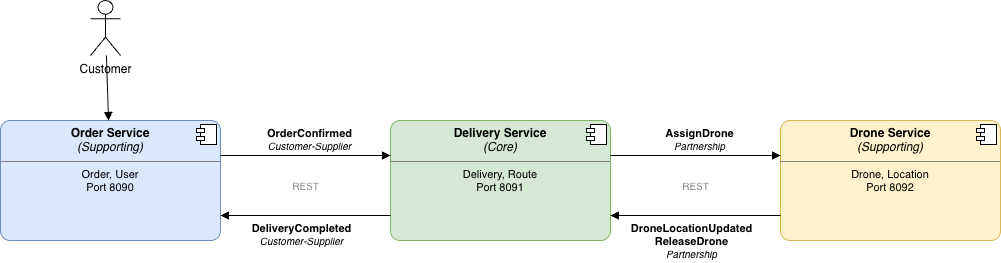
\includegraphics[width=\textwidth]{../doc/design/context-map.png}
\caption{Context Map: relazioni tra Bounded Contexts}
\label{fig:context-map}
\end{figure}

\begin{table}[H]
\centering
\small
\begin{tabularx}{\textwidth}{llX}
\toprule
\textbf{Relazione} & \textbf{Pattern} & \textbf{Comunicazione} \\
\midrule
Order $\to$ Delivery & Customer-Supplier & Order pubblica OrderConfirmed, Delivery reagisce \\
Delivery $\to$ Order & Customer-Supplier & Delivery pubblica DeliveryCompleted, Order reagisce \\
Delivery $\to$ Drone & Partnership & Delivery richiede assegnazione drone via REST \\
Drone $\to$ Delivery & Partnership & Drone pubblica DroneLocationUpdated \\
\bottomrule
\end{tabularx}
\caption{Pattern di integrazione tra Bounded Contexts}
\end{table}

In Assignment 1, tutte le interazioni sono implementate come chiamate REST sincrone tramite proxy adapter, senza event broker.

% ============================================================
\section{Design Tattico (DDD)}
% ============================================================

Il design tattico definisce i building blocks all'interno di ogni Bounded Context.

\subsection{Building Blocks utilizzati}

\begin{table}[H]
\centering
\begin{tabularx}{\textwidth}{lX}
\toprule
\textbf{Building Block} & \textbf{Descrizione} \\
\midrule
Entity & Oggetto con identit\`a persistente (es. \texttt{Order}, \texttt{User}) \\
Value Object & Oggetto senza identit\`a, definito dai suoi attributi, immutabile (es. \texttt{Address}, \texttt{Location}) \\
Aggregate & Cluster di Entity e VO trattati come unit\`a per data modification. Una transazione = un aggregate. \\
Aggregate Root & Unico punto di accesso all'aggregate dall'esterno (es. \texttt{Order}, \texttt{Delivery}, \texttt{Drone}) \\
Domain Event & Notifica immutabile di qualcosa di significativo accaduto nel dominio (es. \texttt{OrderConfirmed}) \\
Repository & Astrazione per accedere agli aggregate come collection in-memory \\
\bottomrule
\end{tabularx}
\caption{Building Blocks DDD utilizzati nel progetto}
\end{table}

\subsection{Marker Interfaces e Annotations}

I building blocks DDD e i concetti dell'architettura esagonale sono resi espliciti nel modulo \texttt{common/}.

I building blocks DDD sono \textbf{interfacce}, perch\'e definiscono comportamento (es. \texttt{getId()}):

\begin{lstlisting}[language=Java]
public interface Entity<T> { T getId(); }
public interface Aggregate<T> extends Entity<T> {}
public interface ValueObject {}
public interface DomainEvent {}
public interface Repository {}
\end{lstlisting}

I ruoli dell'architettura esagonale sono \textbf{annotazioni}, perch\'e sono puri metadata senza comportamento:

\begin{lstlisting}[language=Java]
public @interface InBoundPort {}
public @interface OutBoundPort {}
public @interface Adapter {}
\end{lstlisting}

Questa distinzione permette di verificare automaticamente con ArchUnit che le classi annotate \texttt{@InBoundPort} e \texttt{@OutBoundPort} risiedano nel layer application, e che le classi \texttt{@Adapter} risiedano nel layer infrastructure.

\subsection{Domain Events}

\begin{table}[H]
\centering
\begin{tabularx}{\textwidth}{llX}
\toprule
\textbf{Bounded Context} & \textbf{Evento} & \textbf{Effetto} \\
\midrule
Order & OrderConfirmed & Delivery Service crea una nuova delivery \\
Order & OrderCancelled & Drone viene rilasciato \\
Delivery & DeliveryCompleted & Order passa a COMPLETED, drone rilasciato \\
Delivery & DeliveryFailed & Notifica di fallimento \\
Drone & DroneLocationUpdated & Delivery aggiorna posizione tracking \\
Drone & DroneStatusChanged & Aggiornamento stato flotta \\
\bottomrule
\end{tabularx}
\caption{Domain Events e loro effetti cross-context}
\end{table}

% ============================================================
\section{Architettura}
% ============================================================

\subsection{Stile architetturale: Microservizi}

Lo stile architetturale adottato \`e quello a \textbf{microservizi}, con domain partitioning guidato dal DDD. Ogni microservizio costituisce un \textit{architecture quantum} indipendente: deploy indipendente, database proprio, alta coesione funzionale.

\begin{enumerate}
    \item Identificazione delle system operations (dai requisiti funzionali)
    \item Identificazione dei servizi (dai Bounded Contexts del DDD)
    \item Definizione delle API di ogni servizio (commands, queries, events)
\end{enumerate}

La Figura~\ref{fig:architecture} mostra l'architettura complessiva del sistema.

\begin{figure}[H]
\centering
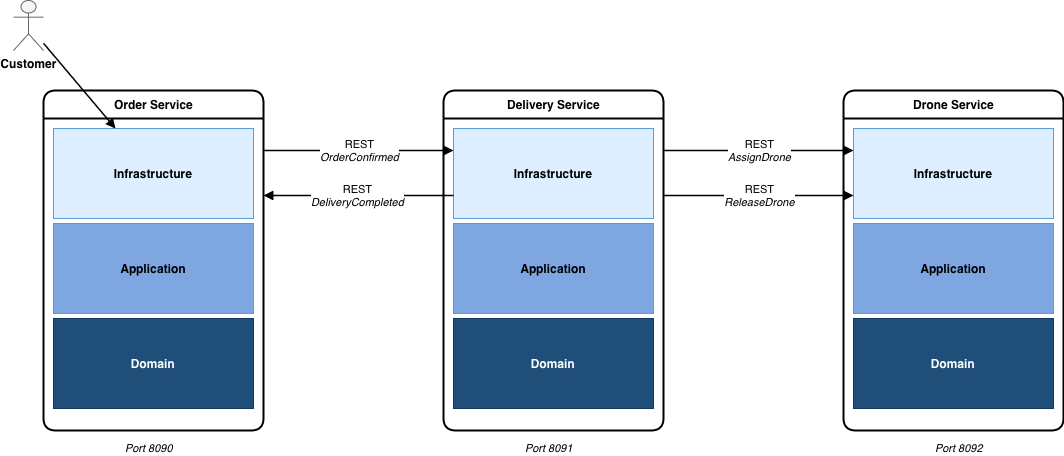
\includegraphics[width=\textwidth]{../doc/design/architecture.png}
\caption{Architettura a microservizi con Clean Architecture interna e comunicazione REST}
\label{fig:architecture}
\end{figure}

\subsection{Architettura interna: Clean/Hexagonal Architecture}

Ogni microservizio segue la \textbf{Clean Architecture}, con tre layer:

\begin{itemize}
    \item \textbf{Domain} (cerchio interno) --- Entities, Value Objects, Aggregates, Domain Events. Nessuna dipendenza verso l'esterno.
    \item \textbf{Application} (cerchio intermedio) --- Use Cases (InBound Ports), interfacce Repository e Service Ports (OutBound Ports). Dipende solo dal domain.
    \item \textbf{Infrastructure} (cerchio esterno) --- Controller REST (Adapter), implementazioni Repository in-memory (Adapter), Proxy Adapter verso altri servizi. Dipende da application e domain.
\end{itemize}

\subsubsection{La Dependency Rule}

Le dipendenze del codice sorgente puntano \textbf{solo verso l'interno}:
\begin{itemize}
    \item \texttt{domain} non importa nulla da \texttt{application} o \texttt{infrastructure}
    \item \texttt{application} importa da \texttt{domain} ma non da \texttt{infrastructure}
    \item \texttt{infrastructure} importa sia da \texttt{application} che da \texttt{domain}
\end{itemize}

L'attraversamento dei confini avviene tramite \textbf{Dependency Inversion}: l'application layer definisce un'interfaccia (OutBound Port), l'infrastructure layer la implementa (Adapter).

La Figura~\ref{fig:cc-internal} mostra il diagramma UML Component \& Connector con la struttura interna di ogni servizio, evidenziando porte e adapter.

\begin{figure}[H]
\centering
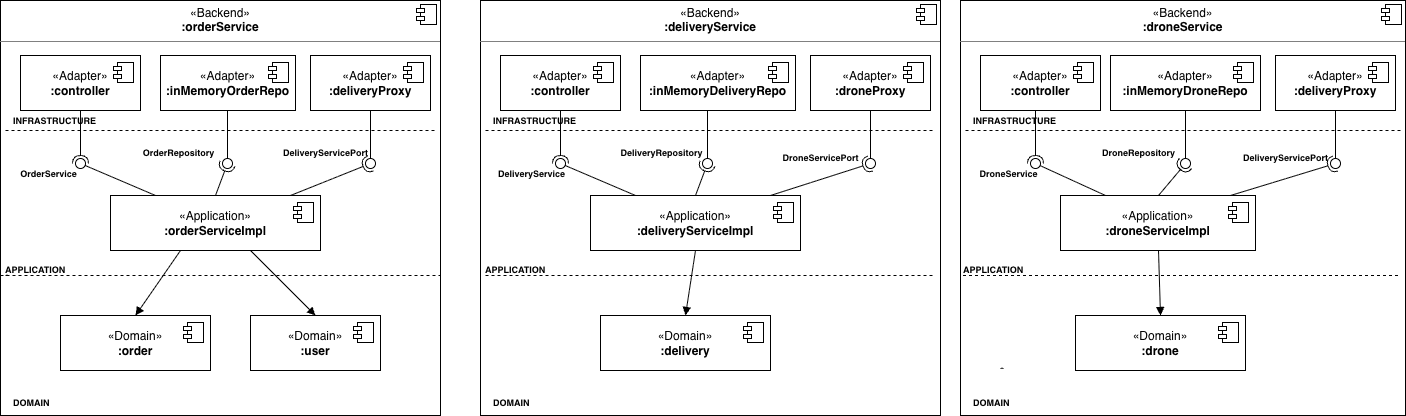
\includegraphics[width=\textwidth]{../doc/design/cc-internal.png}
\caption{Diagramma C\&C: struttura interna dei microservizi con porte e adapter}
\label{fig:cc-internal}
\end{figure}

\subsubsection{Fitness Functions (ArchUnit)}

La Dependency Rule \`e verificata automaticamente tramite \textbf{ArchUnit} (fitness functions strutturali). Due test per ogni servizio:

Il test \texttt{cleanArchitecture()} verifica la layered architecture:

\begin{lstlisting}[language=Java]
var layeredRule = layeredArchitecture()
    .consideringAllDependencies()
    .layer("Domain").definedBy("..domain..")
    .layer("Application").definedBy("..application..")
    .layer("Infrastructure").definedBy("..infrastructure..")
    .whereLayer("Infrastructure").mayNotBeAccessedByAnyLayer()
    .whereLayer("Application").mayOnlyBeAccessedByLayers("Infrastructure")
    .whereLayer("Domain").mayOnlyBeAccessedByLayers("Application", "Infrastructure");
\end{lstlisting}

Il test \texttt{hexagonalArchitecture()} verifica il posizionamento dei ruoli esagonali:

\begin{lstlisting}[language=Java]
var portsRule = classes().that()
    .areAnnotatedWith(InBoundPort.class).or()
    .areAnnotatedWith(OutBoundPort.class)
    .should().resideInAPackage("..application..")
    .orShould().resideInAPackage("..domain..");

var adaptersRule = classes().that()
    .areAnnotatedWith(Adapter.class)
    .should().resideInAPackage("..infrastructure..");
\end{lstlisting}

\subsection{Comunicazione inter-servizio: Proxy Adapter}

La comunicazione tra servizi segue il pattern \textbf{Proxy Adapter}:

\begin{enumerate}
    \item L'application layer definisce un'interfaccia OutBound Port (es. \texttt{DroneServicePort})
    \item L'infrastructure layer implementa un adapter che effettua chiamate REST HTTP al servizio remoto (es. \texttt{DroneServiceProxy})
    \item Il servizio chiamante non conosce i dettagli di comunicazione, li decide l'adapter
\end{enumerate}

Questo rispetta la Dependency Rule: il flusso di controllo va verso l'esterno (verso il servizio remoto), ma le dipendenze del codice puntano verso l'interno (l'adapter dipende dall'interfaccia definita nell'application layer).

% ============================================================
\section{Implementazione}
% ============================================================
\subsection{API REST}

\begin{table}[H]
\centering
\small
\begin{tabularx}{\textwidth}{lllX}
\toprule
\textbf{Servizio} & \textbf{Metodo} & \textbf{Endpoint} & \textbf{Descrizione} \\
\midrule
Order & POST & /api/users/register & Registrazione utente \\
Order & POST & /api/users/login & Login utente \\
Order & POST & /api/orders & Creazione ordine \\
Order & POST & /api/orders/:id/confirm & Conferma ordine \\
Order & POST & /api/orders/:id/cancel & Cancellazione ordine \\
Order & GET & /api/orders/:id & Dettaglio ordine \\
\midrule
Delivery & POST & /api/deliveries & Schedula delivery \\
Delivery & POST & /api/deliveries/:id/start & Avvia transito \\
Delivery & POST & /api/deliveries/:id/complete & Completa delivery \\
Delivery & GET & /api/deliveries/:id & Tracking delivery \\
Delivery & GET & /api/deliveries/order/:orderId & Cerca per ordine \\
\midrule
Drone & POST & /api/drones & Registra drone \\
Drone & GET & /api/drones/available & Trova drone disponibile \\
Drone & POST & /api/drones/:id/location & Aggiorna posizione \\
Drone & POST & /api/drones/:id/release & Rilascia drone \\
Drone & GET & /api/drones/:id & Dettaglio drone \\
\bottomrule
\end{tabularx}
\caption{API REST dei tre microservizi}
\end{table}

Ogni servizio espone una specifica \textbf{OpenAPI 3.0} (\texttt{/api/openapi.yaml}) e un'interfaccia interattiva \textbf{Swagger UI} (\texttt{/swagger-ui}) che permette di esplorare e testare le API direttamente dal browser.

\subsection{Esempio di flusso}

La Figura~\ref{fig:sequence} mostra il diagramma di sequenza del flusso principale.

\begin{figure}[H]
\centering
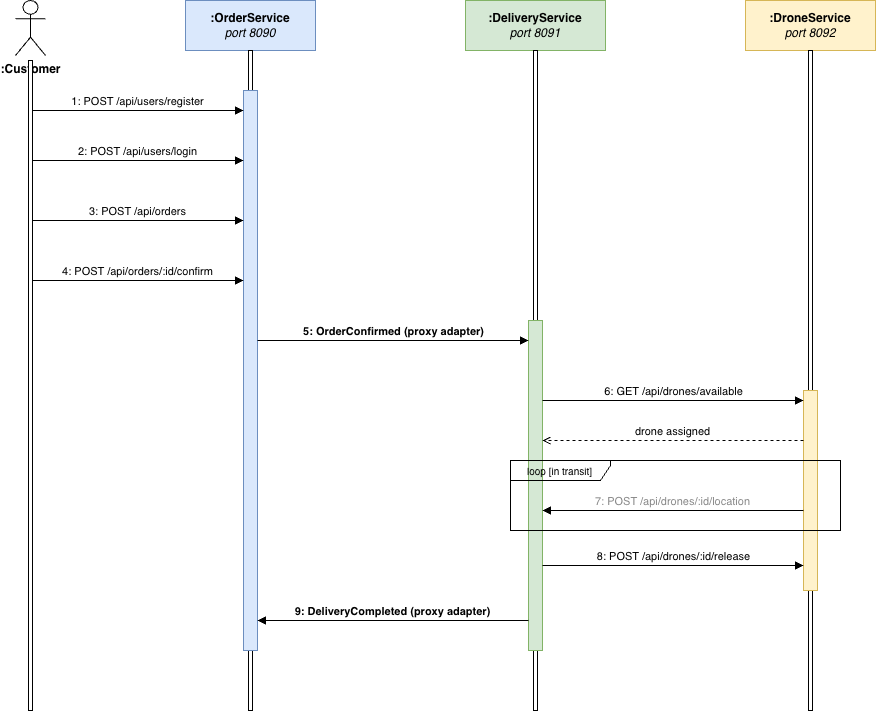
\includegraphics[width=\textwidth]{../doc/design/sequence-flow.png}
\caption{Diagramma di sequenza del flusso principale di consegna}
\label{fig:sequence}
\end{figure}

Il flusso principale del sistema:

\begin{enumerate}
    \item Il \textbf{Customer} registra un account e effettua il login (Order Service)
    \item Il Customer crea un \textbf{Delivery Order} specificando pickup, delivery e peso (Order Service)
    \item Il Customer \textbf{conferma} l'ordine (Order Service)
    \item L'Order Service notifica il Delivery Service tramite \textbf{proxy adapter} (evento OrderConfirmed)
    \item Il Delivery Service crea una \textbf{Delivery} e richiede un drone al Drone Service
    \item Il Drone Service assegna il \textbf{drone pi\`u vicino} con capacit\`a sufficiente
    \item Il drone aggiorna la sua \textbf{posizione} durante il transito
    \item Al raggiungimento della destinazione, la delivery viene \textbf{completata}
    \item Il Delivery Service notifica l'Order Service (evento DeliveryCompleted) e rilascia il drone
\end{enumerate}

% ============================================================
\section{Conclusioni}
% ============================================================

Il progetto dimostra l'applicazione integrata dei concetti studiati nel corso:

\begin{itemize}
    \item Il \textbf{DDD strategico} ha guidato la decomposizione del dominio in subdomains e Bounded Contexts, determinando i confini dei microservizi.
    \item Il \textbf{DDD tattico} ha definito i building blocks interni a ogni servizio (Aggregates, Entities, Value Objects, Domain Events, Repositories).
    \item La \textbf{Clean/Hexagonal Architecture} ha strutturato ogni servizio in layer con la Dependency Rule, garantendo l'indipendenza del dominio dai dettagli tecnici.
    \item I \textbf{Proxy Adapters} hanno implementato la comunicazione inter-servizio rispettando il Dependency Inversion Principle.
    \item Le \textbf{fitness functions} (ArchUnit) verificano automaticamente il rispetto della Dependency Rule.
\end{itemize}

Ogni scelta architetturale \`e motivata dai Quality Attribute Scenarios: la decomposizione a microservizi favorisce \textit{scalability} e \textit{deployability}; la Clean Architecture favorisce \textit{modifiability} e \textit{testability}; il domain partitioning (vs. technical partitioning) allinea l'architettura al dominio di business.

\end{document}
